\documentclass[glossy]{beamer}
\useoutertheme{wuerzburg}
\useinnertheme[realshadow,corners=2pt,padding=2pt]{chamfered}
\usecolortheme{shark}
\graphicspath{ {./Images/} }

\usepackage{tikz}
\newcommand<>{\hover}[1]{\uncover#2{%
 \begin{tikzpicture}[remember picture,overlay]%
 \draw[fill,opacity=0.4] (current page.south west)
 rectangle (current page.north east);
 \node at (current page.center) {#1};
 \end{tikzpicture}}
}

\title{The Art of the C Programming Language}
\author{Natalia Marquez}
\institute{The Institute for Computing in Research}
\date{\today}

\begin{document}

\begin{frame}
\maketitle
\end{frame}

\section{What is C?}
\begin{frame}\centering
  \frametitle{What is C?}
  \includegraphics[scale = 0.50]{DennisRitchie.png}
\end{frame}

\section{The Basics}
\begin{frame}\centering\Huge
  \frametitle{The Basics of C}
  printf(``hello world''); \\~\\
  // Each part of the code above has a meaning
\end{frame}

\section{Variables and Operators}
\begin{frame}\centering\Huge
  \frametitle{Variables}
  int, float, double, and char
\end{frame}
\begin{frame}\centering
  \frametitle{Operators}
  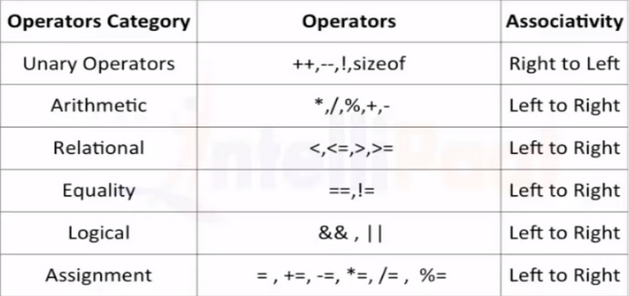
\includegraphics[scale = 0.5]{Operators.png}
\end{frame}

\section{Functions and Structures}
\begin{frame}\centering
  \frametitle{Functions}
  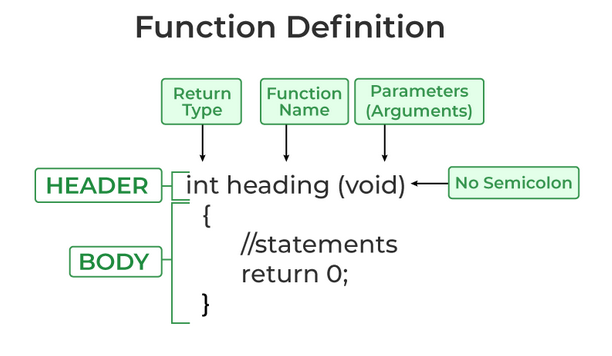
\includegraphics[scale = 0.5]{Function.png}
\end{frame}
\begin{frame}\centering
  \frametitle{Structures}
  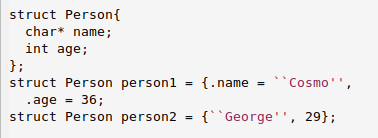
\includegraphics[scale = 0.75]{Structures.png}
\end{frame}

\section{Conditionals and Loops}
\begin{frame}\centering
  \frametitle{Conditionals}
  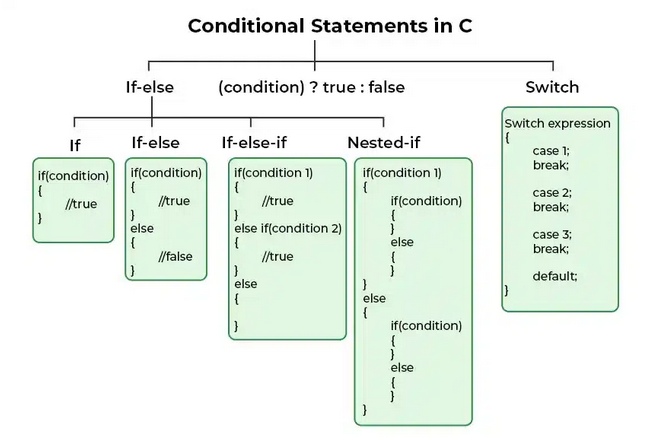
\includegraphics[scale = 0.45]{Conditionals.png}
\end{frame}
\begin{frame}\centering
  \frametitle{Loops}
  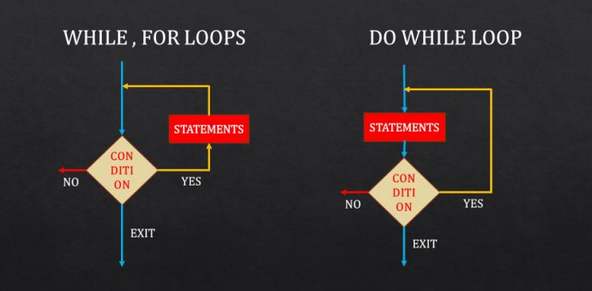
\includegraphics[scale = 0.55]{Loops.png}
\end{frame}

\section{Arrays and Strings}
\begin{frame}\centering
  \frametitle{Arrays}
  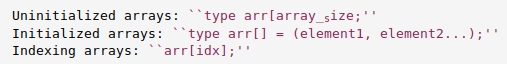
\includegraphics[scale = 0.65]{Arrays.png}
\end{frame}
\begin{frame}\centering\Huge
  \frametitle{Strings}
  strlen() \\~\\
  strcat() \\~\\
  strcpy()
\end{frame}

\section{Pointers}
\begin{frame}\centering
  \frametitle{Pointers}
  \includegraphics[scale = 0.5]{Pointers.jpeg} \\~\\
  type* pntr; or type *pntr;
\end{frame}

\section{Acknowledgements}
\begin{frame}\centering\Huge
  Thank you!
\end{frame}

\end{document}
